% Lemoine 猜想数值研究论文（目标期刊：Integers / J. Integer Seq. / Exp. Math.）
% 编译：pdflatex main.tex
\documentclass[11pt]{article}
\usepackage{amsmath,amssymb,amsthm}
\usepackage{graphicx}
\usepackage{booktabs}
\usepackage[margin=1.1in]{geometry}
\usepackage{hyperref}

\newtheorem{conjecture}{Conjecture}
\newtheorem{heuristic}{Heuristic}

\title{Exhaustive Verification, Minimal-Prime Records, and\\
Representation Statistics for Lemoine's Conjecture}
\author{Yunyue Li}
\date{\today}

\begin{document}
\maketitle

\begin{abstract}
Lemoine's conjecture (1895) asserts that every odd integer $n>5$ can be
written as $n=p+2q$ with $p,q$ prime. We report an exhaustive verification
for all odd $n \le 2\times10^{13}$ (no counterexample; 19 hours on eight
consumer cores),
computing simultaneously the record values of the minimal doubled prime
($n=p+2q$, minimal $q$) and of the minimal undoubled prime ($n=2p+q$,
minimal $q$), the latter cross-validating --- and extending by one
term --- the OEIS sequence A002091.
Using FFT convolution we further compute the exact representation function
$r(n)=\#\{(p,q):n=p+2q\}$ for every odd $n\le 10^{7}$, extended by
windowed exact counts up to $10^{8}$, confirming a
Hardy--Littlewood-type asymptotic $r(n)\approx 2C_2\,K(n)\,I(n)$ with
singular series factor $K(n)=\prod_{\ell\mid n,\,\ell>2}\frac{\ell-1}{\ell-2}$.
The normalized deviation $2C_2 - r(n)/(K(n)I(n))$ decays as a power law
$c\,n^{-\theta}$ with $\theta = 0.519 \pm 0.007$ over almost four decades,
consistent with square-root cancellation ($\theta=\tfrac12$) as expected
from the explicit formula, while a $1/\log n$ correction model is excluded
($\chi^2/\mathrm{dof} \approx 11$). A weighted periodogram of the
power-law residuals detects the oscillatory contributions of the
low-lying nontrivial zeros of the Riemann zeta function directly in the
Lemoine representation data. All code and data are open source.
\end{abstract}

\section{Introduction}

Lemoine's conjecture, independently restated by Levy \cite{levy}, asserts:

\begin{conjecture}[Lemoine 1895]
Every odd integer $n>5$ admits a representation $n = p + 2q$ with $p$, $q$ prime.
\end{conjecture}

The conjecture is formally stronger than the weak Goldbach conjecture
(proved by Helfgott \cite{helfgott}): summing $p$ and $q$ twice gives a
three-prime representation of $n$. Unlike the even Goldbach conjecture,
whose empirical verification has reached $4\times10^{18}$
\cite{oesilva}, the computational status of Lemoine's conjecture is
scattered: MathWorld credits Corbitt with a verification to $10^9$
\cite{mathworld-levy}; a 2019 blog post reports $10^{10}$
\cite{brainhappy}; and a 2011 comment on OEIS A002091 by Pfoertner
reports the record values of the associated minimal-prime sequence up to
$10^{13}$ \cite{oeis2091}, which implies (but nowhere formally documents)
a verification to that bound. A recent article \cite{ndegwa} tests
randomly sampled odd integers of up to 1500 digits by probabilistic
primality testing; such spot checks, while consistent with the
conjecture, do not establish an exhaustive bound. A claimed proof
\cite{agama} was later found to be flawed; the conjecture remains open. Zhang \cite{zhang} studies an
equivalent form of a strong version of the conjecture; another claimed
proof \cite{ghanim} has not gained acceptance.

Our contributions: (i) a single reproducible exhaustive verification to
$2\times10^{13}$, producing both minimal-prime record sequences, one of
which reproduces the full A002091 $b$-file and extends it by one term; (ii) exact representation counts $r(n)$
for all odd $n\le10^7$ via FFT convolution; (iii) a numerical test of the
Hardy--Littlewood-type asymptotic, including the first (to our knowledge)
empirical determination of the decay exponent of its second-order term;
(iv) open-source, single-machine code: verification to $10^{12}$ takes
under one hour on a consumer laptop, and to $2\times10^{13}$ under a day.

\section{A Hardy--Littlewood heuristic for $r(n)$}\label{sec:heuristic}

Model the primality of the two components independently: an integer of
size $t$ is prime with ``probability'' $1/\log t$. For odd $n$ and a
random $q \in [3, (n-3)/2]$, set $p = n - 2q$. The naive expectation is
$I(n) = \sum_{q=3}^{(n-3)/2} \frac{1}{\log q\,\log(n-2q)}$.
Local corrections at each prime $\ell$ multiply this by
\[
\delta_\ell =
\frac{\Pr[\ell \nmid q \text{ and } \ell \nmid n-2q]}{\Pr[\ell\nmid q]\Pr[\ell\nmid p]}.
\]
For $\ell = 2$: $p = n-2q$ is automatically odd, so $\delta_2 = 2$.
For odd $\ell \nmid n$: the events $\ell \mid q$ and $\ell \mid n-2q$
concern two distinct residues of $q$, giving
$\delta_\ell = (1-2/\ell)/(1-1/\ell)^2 = 1 - 1/(\ell-1)^2$.
For odd $\ell \mid n$: here $\ell \nmid n-2q$ holds automatically
whenever $\ell \nmid q$, so the joint probability is $1-1/\ell$ and
$\delta_\ell = (1-1/\ell)/(1-1/\ell)^2 = \ell/(\ell-1)$.
Writing the full product over the factors $1-1/(\ell-1)^2$ and
correcting at $\ell \mid n$ by
$\frac{\ell/(\ell-1)}{1-1/(\ell-1)^2} = \frac{\ell-1}{\ell-2}$, we obtain
\[
r(n) \;\approx\; 2C_2\,K(n)\,I(n),
\qquad
K(n) = \prod_{\ell\mid n,\ \ell>2}\frac{\ell-1}{\ell-2},
\qquad
C_2 = \prod_{\ell>2}\Bigl(1-\frac{1}{(\ell-1)^2}\Bigr) \approx 0.66016,
\]
the exact analogue of Hardy--Littlewood's Conjecture~A for Goldbach's
problem \cite{hl}, with the same twin-prime constant and singular series.

\section{Exhaustive verification and minimal-prime records}\label{sec:verify}

\subsection{Algorithm}
Segmented odd-only bitmap sieve; for each odd $n$ we search the minimal
$q$ (list of primes $q < 2\times10^5$) with $n-2q$ prime, using a window
extending $2\times10^5$ below the segment. A second window at half height
serves the mirrored decomposition $n = 2p+q$. Eight threads; segment
length $2^{28}$. Work is dominated by the segmented sieving,
$O(N\log\log N)$ bit operations overall with $O(\sqrt N)$ memory for the
base primes plus $O(1)$ per-thread window bitmaps (32\,MB each); the
decomposition search itself averages fewer than four primality lookups
per $n$. The $10^{10}$ prefix agrees with an independent non-segmented
implementation.

\subsection{Results}
No counterexample exists below $2\times10^{13}$: every odd
$7 \le n \le 2\times10^{13}$ admits both decompositions $n=p+2q$ and
$n=2p+q$. The full run took 68\,941 seconds ($\approx19$ hours) on eight
performance cores of a consumer laptop (Apple M-series); a $10^{12}$ run
takes 3314 seconds. The minimal doubled prime attains its maximum
$q_{\min} = 4261$ at $n = 19\,909\,053\,765\,571$ (45 record values in
total; Table~1 shows the tail), and the minimal undoubled prime attains
$q_{\min} = 9157$ at $n = 14\,480\,831\,322\,263$ (50 records). The
noncomposite variant of the undoubled-side record sequence reproduces
the OEIS A002091 $b$-file exactly --- all 49 published terms, which
reach $8\,567\,125\,268\,699$ --- providing a full independent
cross-validation of both computations, and extends the sequence by one
new term,
\[
a(50) = 12\,279\,230\,664\,247, \qquad q_{\min} = 8969.
\] Complete record lists and the $q_{\min}$
distribution histograms are provided in the repository.

\begin{table}[ht]\centering
\caption{Record values of the minimal prime $q$: left, in $n=p+2q$
(45 records below $2\times10^{13}$, tail shown); right, in $n=2p+q$
(50 records, tail shown).}
\begin{tabular}{rr@{\qquad}rr}
\toprule
$n$ & $q_{\min}$ & $n$ & $q_{\min}$ \\
\midrule
646\,341\,033\,061 & 2971 & 2\,695\,682\,504\,171 & 8017 \\
853\,036\,242\,229 & 3079 & 5\,947\,609\,572\,643 & 8597 \\
10\,154\,135\,153\,999 & 3851 & 8\,567\,125\,268\,699 & 8821 \\
13\,982\,148\,897\,511 & 3907 & 12\,279\,230\,664\,247 & 8969 \\
18\,115\,451\,658\,709 & 4093 & 14\,480\,831\,322\,263 & 9157 \\
19\,909\,053\,765\,571 & 4261 & & \\
\bottomrule
\end{tabular}
\end{table}

\subsection{Growth of the records and the random model}
In a Cram\'er-type model the probability that a fixed candidate prime
$q$ fails for a given $n$ is $1 - O(K(n)/\log n)$, so
$\Pr[q_{\min} > Q] \approx \exp(-c\,K(n)\,\pi(Q)/\log n)$ and record
values should satisfy $\pi(q_{\min}) \asymp \alpha (\log n)^2$ up to
$\log\log$ factors. The data agree: a one-parameter fit through the
records with $n > 10^3$ gives $\alpha_A = 0.60$ (28 records) for
$n = p+2q$ and $\alpha_B = 1.17$ (34 records) for $n = 2p+q$. The ratio
$\alpha_B/\alpha_A = 1.94 \approx 2$ has a clean explanation: in
$n = p+2q$ the residual $p = n-2q$ is forced to be odd, doubling its
chance of primality, whereas $p = (n-q)/2$ in the mirrored decomposition
carries no parity constraint; the per-candidate success probability
halves and the record threshold in $\pi(Q)$ doubles.



\section{Exact representation counts via FFT}\label{sec:fft}

$r(n)$ for all odd $n \le 10^7$ is the convolution of the prime indicator
with the doubled-prime indicator, computed exactly by 64-bit-float FFT of
length $2^{25}$ and rounding (max entry $\approx1.3\times10^5$, far below
the $2^{53}$ integer threshold; spot checks against brute force agree).
Figure~\ref{fig:comet} shows the Lemoine comet near $10^7$: the four
divisibility classes of $n$ by 3 and 5 separate into bands whose heights
follow the singular-series ratios $1 : \tfrac43 : 2 : \tfrac83$.

\begin{figure}[ht]\centering
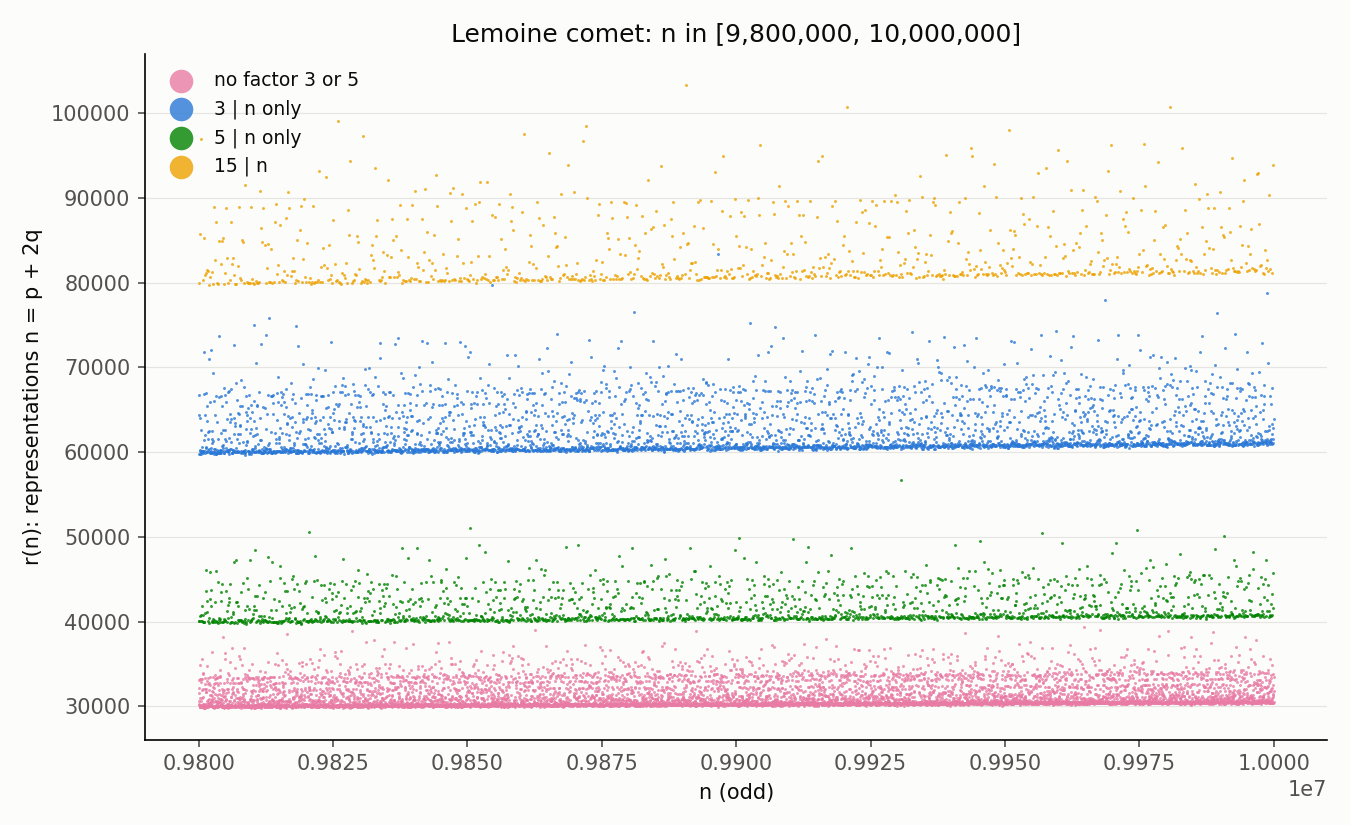
\includegraphics[width=.92\textwidth]{../figures/comet.png}
\caption{The Lemoine comet: $r(n)$ for odd
$n\in[9.8\times10^6,\,10^7]$, stratified by divisibility by 3 and 5.}
\label{fig:comet}
\end{figure}

\section{Testing the asymptotic; the second-order term}\label{sec:second}

Averaging $\rho(n) = r(n)/(K(n)I(n))$ over windows of 500 consecutive odd
integers at 48 log-spaced centers below $10^7$, plus five windows of
exact counts between $10^{7.2}$ and $10^8$ computed by direct windowed
convolution: for $n>10^6$ the mean is
$1.3174\pm0.0046$ against $2C_2 = 1.32032$. The deviation
$g(n) = 2C_2 - \rho(n)$ is positive throughout and decays as
\[
g(n) \;=\; c\,n^{-\theta}, \qquad \theta = 0.519 \pm 0.007,\quad c\approx 5.1,
\]
over almost four decades (Figure~\ref{fig:power}). A first-order logarithmic
model $\rho = a + b/\log n$ is excluded: it extrapolates to
$a = 1.3489\pm0.0006$, $49\sigma$ above $2C_2$, with
$\chi^2/\mathrm{dof} = 10.9$. The exponent $\theta\approx\tfrac12$ is the
signature of square-root cancellation: replacing the $1/\log$ density
model by the explicit formula introduces zero-sum terms of relative size
$n^{-1/2}$ under RH, exactly as in the average theory of Goldbach
representations developed by Languasco and Zaccagnini \cite{lz}.
The residuals about the fitted power law are not white: successive
windows drift coherently, as expected if $g(n)$ carries an oscillatory
factor $\sum_\gamma \cos(\gamma\log n + \phi_\gamma)$ from the nontrivial
zeros $\rho = \tfrac12 + i\gamma$ of $\zeta(s)$.

\subsection{Detecting the zeros}\label{sec:zeros}
To test this directly we densify the sampling to 224 windows
($10^{4.7}$--$10^8$) and compute a weighted least-squares periodogram of
the relative residuals: for each frequency $\gamma$ we fit
$a\cos(\gamma\log n)+b\sin(\gamma\log n)$ and record the $\chi^2$
improvement $\Delta\chi^2(\gamma)$ (2 degrees of freedom; white-noise
expectation 2). Figure~\ref{fig:zeros} shows the result over
$\gamma\in[3,60]$: the dominant peaks of the periodogram coincide with
the ordinates of the low-lying Riemann zeros. The maximum,
$\Delta\chi^2 = 55.5$ at $\gamma = 37.45$, sits at
$\gamma_6 = 37.5862$; distinct peaks also appear at
$\gamma_1, \gamma_2, \gamma_3, \gamma_4, \gamma_8$ and $\gamma_{12}$,
while frequencies away from zeros show near-background power. The summed
power at the first 13 zero ordinates is $219.5$ against a white-noise
expectation of $26$.

\emph{Robustness.} The analysis was repeated with window half-widths
$W=100$ and $W=500$ (baseline $W=250$) and with the discrete sum $I(n)$
replaced by a midpoint-rule integral. The $I(n)$ discretization is
immaterial (periodograms indistinguishable; peak $\Delta\chi^2$ 53.0
vs.\ 53.1). Varying $W$ rescales the signal-to-noise as expected ---
$\Delta\chi^2$ at the zeros grows from $\approx25$ ($W=100$) to
$\approx89$ ($W=500$) --- while peaks remain locked to the zero
ordinates in every configuration; which zero carries the largest power
varies with the weighting, so we do not interpret the relative
amplitudes. The fitted exponent is stable at
$\theta \in [0.517, 0.525]$ across all configurations
(Figure~\ref{fig:robust}).

\emph{Joint fit and trials-corrected significance.}
Fitting all thirteen frequencies simultaneously (fixed at the zero
ordinates; amplitudes and phases free, 26 linear parameters plus the
smooth trend) improves the fit by $\Delta\chi^2 = 258.0$ and reduces
$\chi^2/\mathrm{dof}$ from $2.6$ to $1.64$. To calibrate the look-elsewhere
effect we repeated the identical 13-frequency fit for 500 random
frequency sets drawn uniformly from $[10,60]$ (excluding $\pm1$
neighborhoods of the zeros): the null distribution has mean
$\Delta\chi^2 = 76$ and maximum $124.5$, so the value attained by the
actual zero ordinates exceeds every random trial (empirical
$p < 2\times10^{-3}$, and far smaller by extrapolation of the null
tail). The fitted amplitudes (Figure~\ref{fig:amps}) are of the
magnitude suggested by the explicit formula and broadly follow the
$1/\gamma$ weighting, with two notable outliers ($\gamma_6$ strong,
$\gamma_1$ weak); the transfer function of our windowed, detrended
statistic --- and the residual structure at $\chi^2/\mathrm{dof}=1.64$,
plausibly higher zeros --- remain open questions.

\begin{figure}[ht]\centering
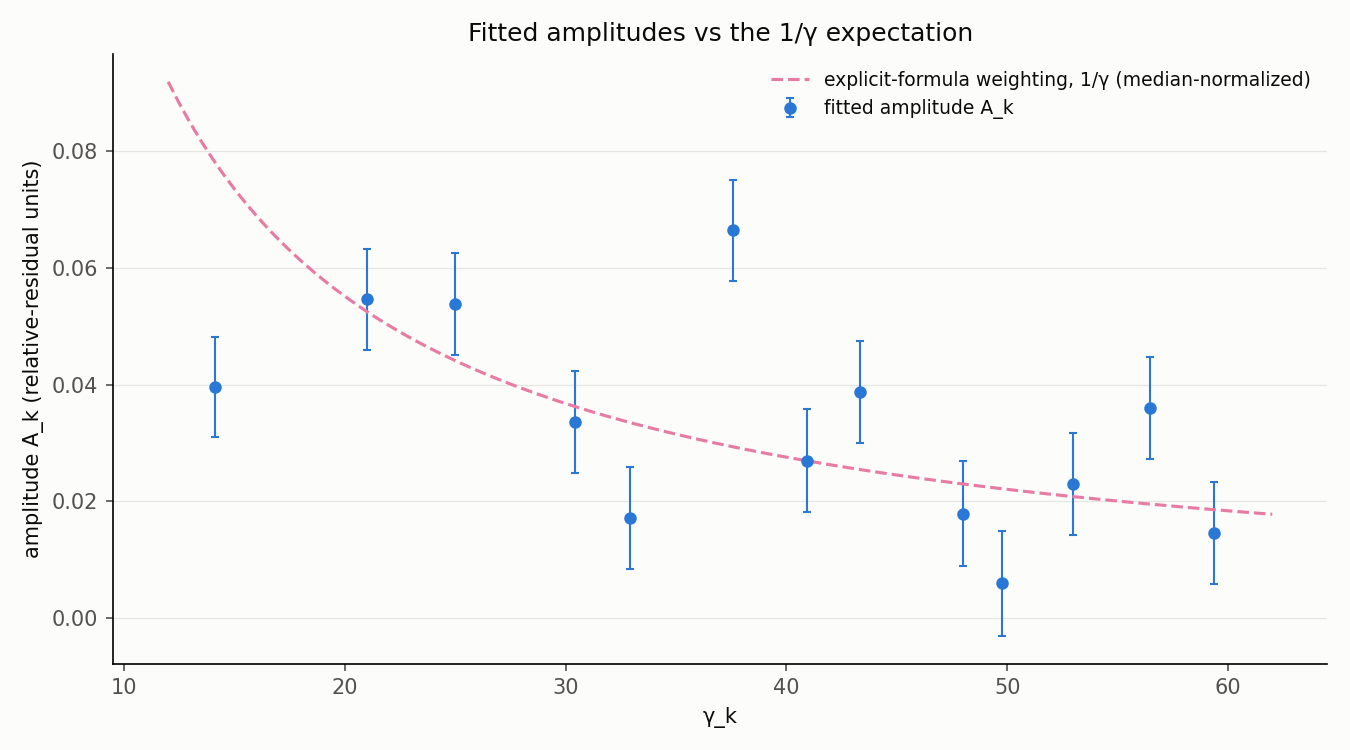
\includegraphics[width=.92\textwidth]{../figures/zero_amplitudes.png}
\caption{Amplitudes of the thirteen fixed-frequency components from the
joint fit, against the $1/\gamma$ weighting suggested by the explicit
formula (dashed; median-normalized).}
\label{fig:amps}
\end{figure}

\begin{figure}[ht]\centering
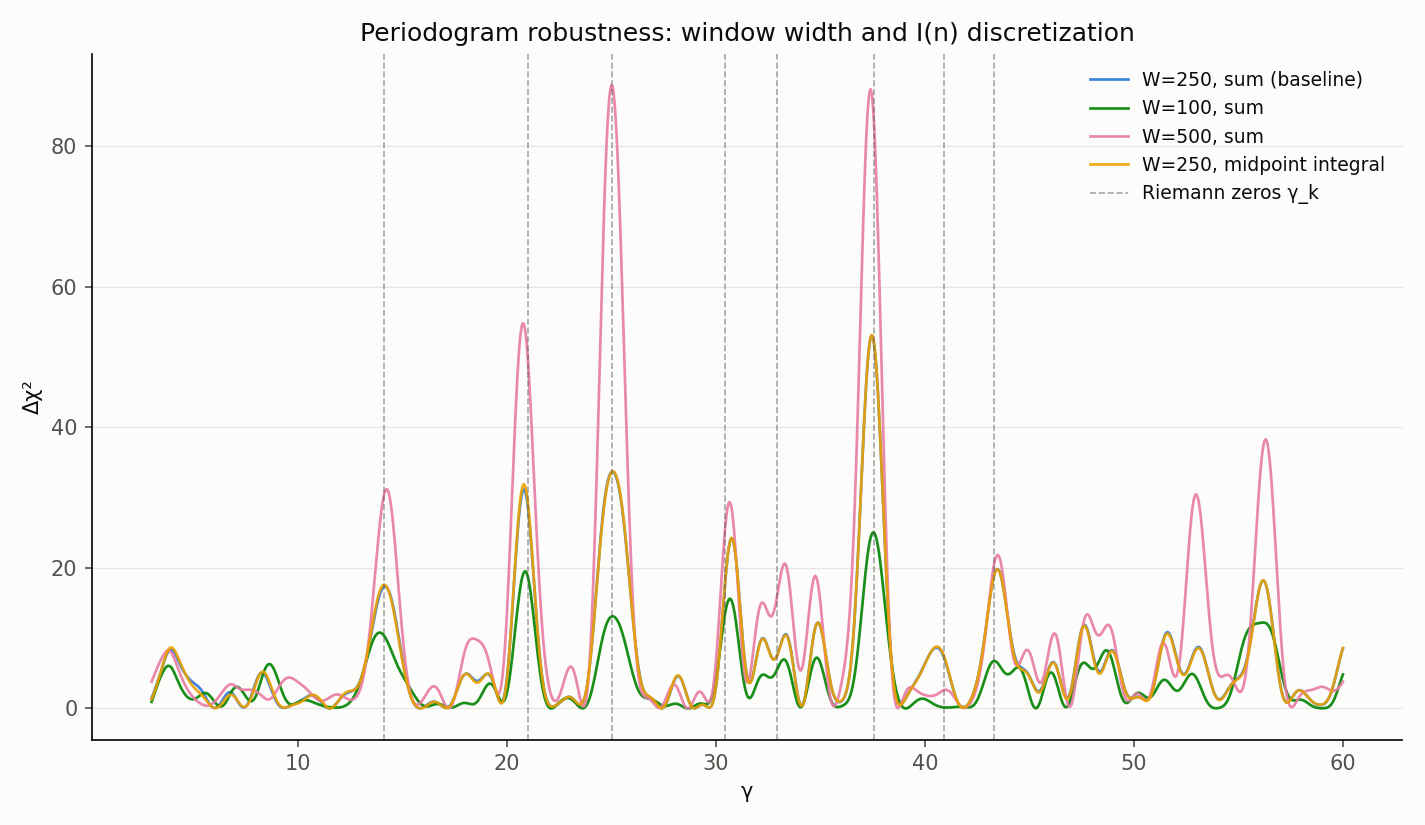
\includegraphics[width=.92\textwidth]{../figures/zero_robustness.png}
\caption{Periodograms under four analysis configurations: window
half-widths $W\in\{100,250,500\}$ and two discretizations of $I(n)$.
Peaks stay locked to the zero ordinates (dashed).}
\label{fig:robust}
\end{figure}

\begin{figure}[ht]\centering
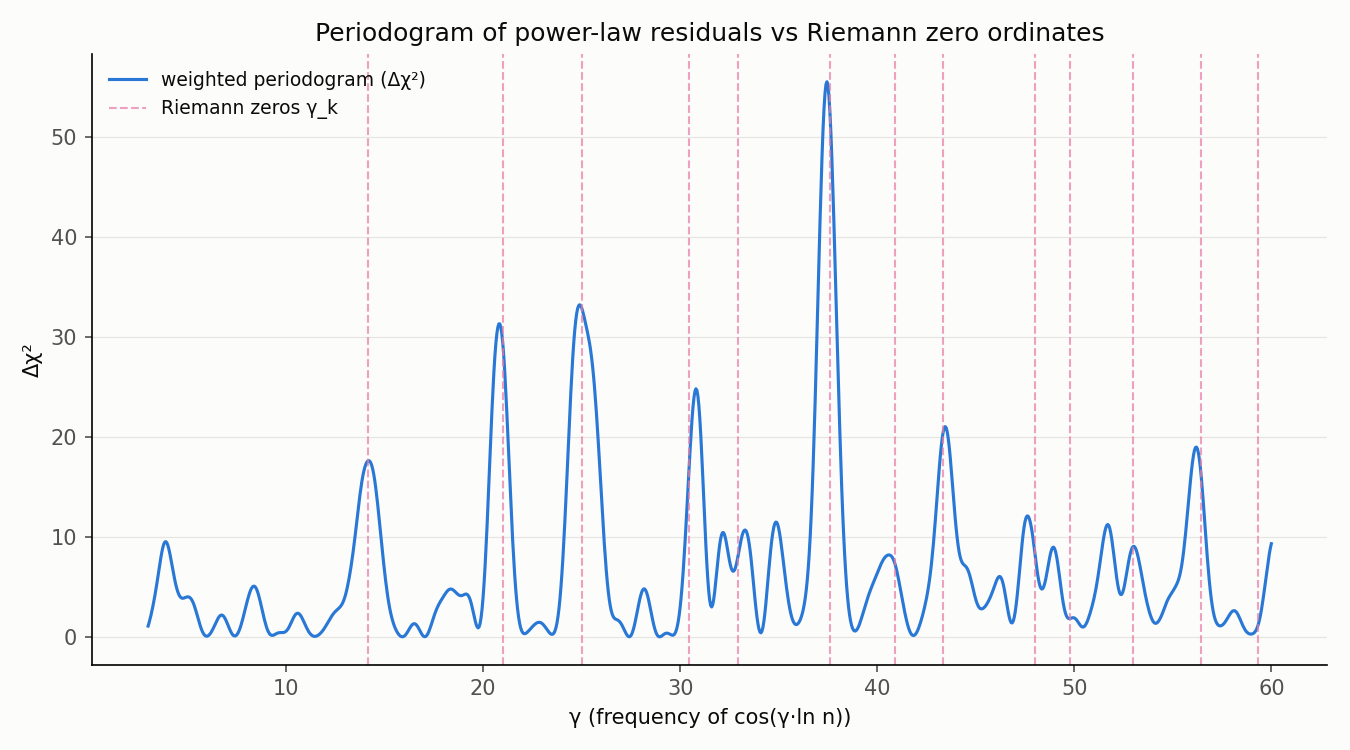
\includegraphics[width=.92\textwidth]{../figures/zero_periodogram.png}
\caption{Weighted periodogram of the power-law residuals of $g(n)$.
Dashed lines mark the ordinates $\gamma_k$ of the first nontrivial zeros
of $\zeta(s)$.}
\label{fig:zeros}
\end{figure}

\begin{figure}[ht]\centering
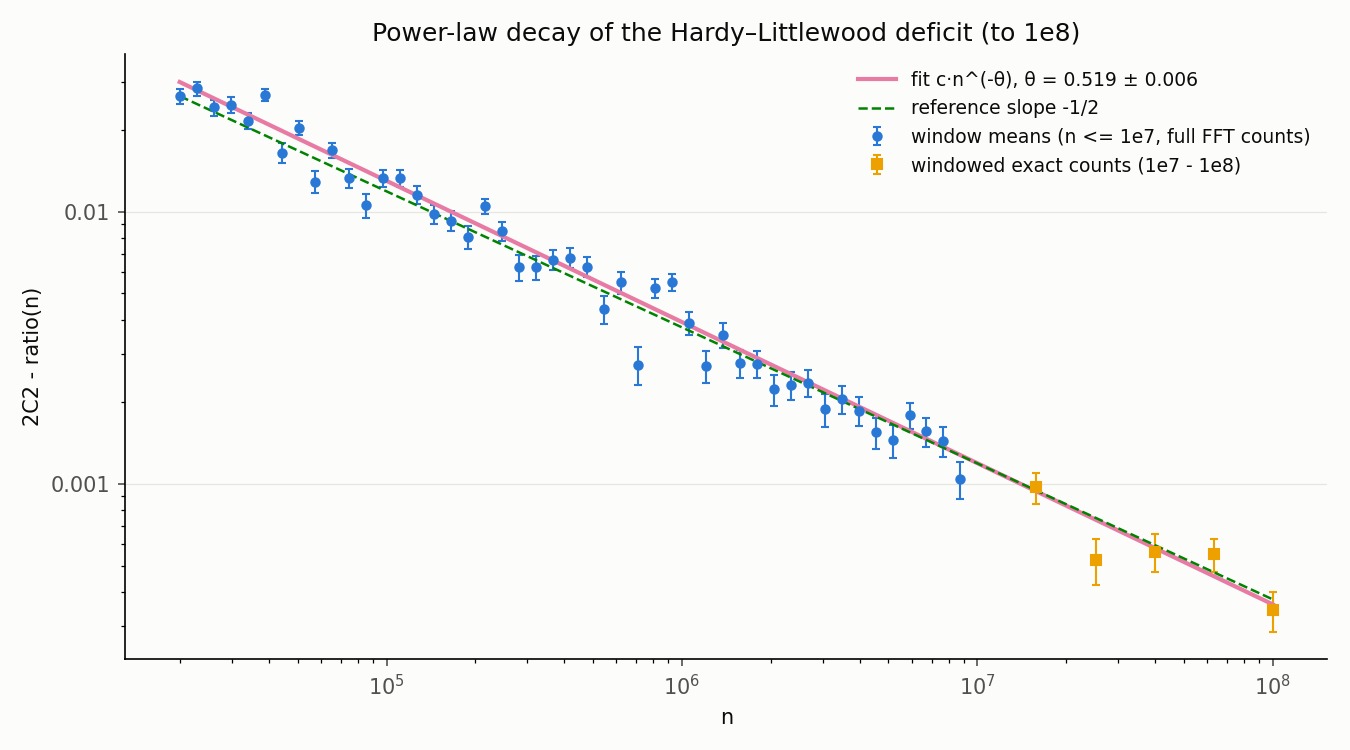
\includegraphics[width=.92\textwidth]{../figures/second_order_1e8.png}
\caption{Power-law decay of the deviation from the Hardy--Littlewood
prediction; the dashed line has slope $-\tfrac12$.}
\label{fig:power}
\end{figure}

\section{Data and code availability}
% GitHub 仓库链接；数据文件清单（记录 CSV、直方图、拟合数据）。

\begin{thebibliography}{99}
\bibitem{lemoine} E. Lemoine, L'interm\'ediaire des math\'ematiciens 1 (1894), 179; 3 (1896), 151.
\bibitem{levy} H. Levy, On Goldbach's conjecture, Math. Gaz. 47 (1963), 274.
\bibitem{hl} G. H. Hardy and J. E. Littlewood, Some problems of `Partitio Numerorum' III, Acta Math. 44 (1923), 1--70.
\bibitem{helfgott} H. A. Helfgott, The ternary Goldbach conjecture is true, arXiv:1312.7748 (2013).
\bibitem{oesilva} T. Oliveira e Silva, S. Herzog, S. Pardi, Empirical verification of the even Goldbach conjecture and computation of prime gaps up to $4\cdot10^{18}$, Math. Comp. 83 (2014), 2033--2060.
\bibitem{mathworld-levy} E. W. Weisstein, Levy's Conjecture, MathWorld.
\bibitem{brainhappy} Lemoine's conjecture verified to $10^{10}$, makethebrainhappy.com, June 2019.
\bibitem{oeis2091} OEIS Foundation, Sequence A002091 (comment by H. Pfoertner, Sep 2011).
\bibitem{ndegwa} D. Ndegwa et al., Extending computational verification of Lemoine's conjecture to 1500 digit odd numbers, IJMTT 72(3) (2026), 49--52.
\bibitem{agama} T. Agama and B. Gensel, A proof of Lemoine's conjecture by circles of partition, arXiv:1709.05335 (2021); flawed, see discussion in the literature.
\bibitem{lz} A. Languasco and A. Zaccagnini, The number of Goldbach representations of an integer, Proc. Amer. Math. Soc. 140 (2012), 795--804.
\bibitem{zhang} S. Zhang, An equivalent form of strong Lemoine conjecture and several relevant results, Wuhan Univ. J. Nat. Sci. 24(3) (2019), 229--232.
\bibitem{ghanim} M. Ghanim, Confirmation of the Lemoine--Levy conjecture, Global J. Adv. Eng. Tech. Sci. 8(12) (2021), 1--7.
\bibitem{oeis46927} OEIS Foundation, Sequence A046927: number of ways to express $2n+1$ as $p+2q$ with $p,q$ prime.
\bibitem{oeis185091} OEIS Foundation, Sequence A185091: smallest positive noncomposite $q$ with $2n-1 = 2p+q$, $p$ noncomposite.
\end{thebibliography}
\end{document}
